\chapter{Graph Adjacency Lists and Matrices}

\setcounter{problem}{1}

\section{Goal}

\begin{fullwidth}

The goal of this task is to teach you about the implementation of graphs in Python, how to implement a few simple related algorithms, and do some simple data loading.  As part of this exercise, you will also learn to transform data, which is an important data preparation skill you will need as an analyst. 

\section{Discussion}

In this project, you will convert a \href{https://raw.githubusercontent.com/parrt/msan501/master/data/graph}{{\textcolor{blue}string representation of a graph}} that looks like this:

\begin{alltt}\small
parrt: tombu, dmose, parrt
tombu: dmose, kg9s
dmose: tombu
kg9s: dmose
\end{alltt}

\noindent to an adjacency list representation and ultimately generate a visual representation via \href{http://www.graphviz.org/}{\textcolor{blue}{graphviz/dot}}:

\begin{center}
\scalebox{.55}{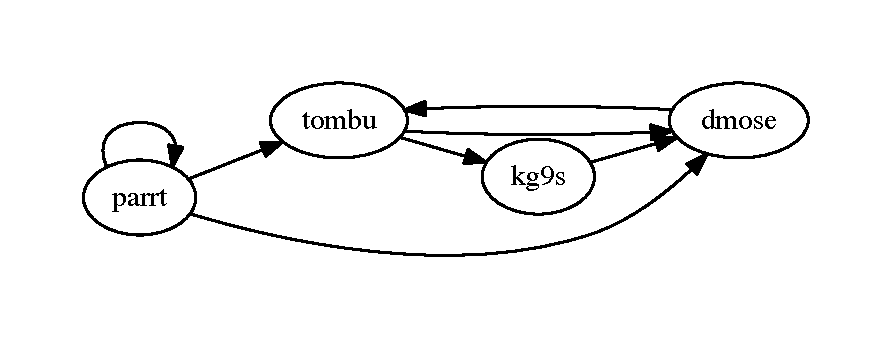
\includegraphics{figures/email-graph.pdf}}
\end{center}

\noindent For fun, you will also create an edge matrix representation:

\[
\bordermatrix{
~ & parrt & tombu & dmose & kg9s \cr
parrt & 1 & 1 & 1 & 0\cr
tombu & 0 & 0 & 1 & 1 \cr
dmose & 0 & 1 & 0 & 0 \cr
kg9s & 0 & 0 & 1 & 0\cr
}
\]

\noindent where the nodes have the following indexes (all we really care about here is the order):
 
\[
\left[
\begin{array}{c}
0: parrt \\
1: tombu \\
2: dmose \\
3: kg9s \\
\end{array}
\right]
\]

The following sections describe the functions you must create in {\tt graphs.py}. Your starter kit should have some boilerplate code set up for you.

\subsection{Processing an adjacency list string}

First, you have to process a string representation of an adjacency list and create an internal data structure:

\begin{pyverbatim}
def adjlist(adj_list):
    """
    Read in adj list and store in form of dict mapping node
    name to list of outgoing edges. Preserve the order you find
    for the nodes.
    """
    ...
\end{pyverbatim}

You will use an ordered dictionary ({\tt OrderedDict}) that maps node name x to a list of target nodes. x will be a string and the target list will be a list of strings. For example, from line in string adj\_list

\begin{alltt}
parrt: tombu, dmose, parrt
\end{alltt}

\noindent you will create an entry in the dictionary with key {\tt parrt} and value:

\begin{pyverbatim}
['tombu', 'dmose', 'parrt']
\end{pyverbatim}

\noindent To process the text, you must split the incoming string into lines and then process them one at a time as each line represents an adjacency list. You will use string functions {\tt split} and (likely) {\tt strip} to process the text. The goal here is to learn how to process text so don't look for built-in functions that do all of this for you.

\noindent Printing the adjacency list dictionary from {\tt adjlist}, we should all get the following output:

\begin{pyverbatim}
OrderedDict([('parrt', ['tombu', 'dmose', 'parrt']),
 ('tombu', ['dmose', 'kg9s']), 
 ('dmose', ['tombu']), 
 ('kg9s', ['dmose'])])
\end{pyverbatim}

\subsection{Adjacency list to adjacency matrix}

Given an adjacency list stored as a dictionary per adjlist(), create a function that converts it to an adjacency matrix:
 
\begin{pyverbatim}
def adjmatrix(adj):
    """
    From an adjacency list, return the adjacency matrix with entries in {0,1}.
    The order of nodes in adj is assumed to be same as they were read in.
    """
    ...
\end{pyverbatim}

\noindent The matrix should look like the one shown above.

\subsection{Getting a list of all nodes}

A very useful function to have is the following that returns a list of all nodes visited starting at a particular node in a graph. 
 
\begin{pyverbatim}
def nodes(adj, start_node):
    """
    Walk every node in graph described by adj list starting at start_node
    using a breadth-first search.  Return a list of all nodes found (in
    any order). Include the start_node.
    """
    ...
\end{pyverbatim}

\noindent Do not build a recursive function as you must do a breadth-first search. (Recursive functions are much more useful when doing a depth-first search.) The basic algorithm looks like this:

\begin{algorithm}[H]
\SetInd{.3em}{.3em}
$visited$ = []\;
add the start node to a work list\;
\While{more work}{
    node = remove a node from work list\;
    add node to $visited$ list\;
    targets = adjacency\_list[node]\;
    add all unvisited targets to work list\;
}
\Return{visited}\;
\end{algorithm}

\subsection{Generating DOT output}

In order to visualize the graph you have read in, create the following function that dumps valid Graphviz DOT code, given an adjacency list. Then cut-and-paste the output and put it into Graphviz to display it.
 
\begin{pyverbatim}
def gendot(adj):
    """
    Return a string representing the graph in Graphviz DOT format
    with all p->q edges. Parameter adj is an adjacency list.
    """
    ...
\end{pyverbatim}

\noindent Or, to amaze your family and friends, you can directly from the command line on a mac or unix box:

\begin{lstlisting}[style=BashInputStyle]
$ python test_dot.py | dot -Tpdf > /tmp/graph.pdf; open /tmp/graph.pdf
\end{lstlisting}

Here is a simple test rig, {\tt test\_dot.py}, that translates an input string description to DOT and prints it out.

\begin{pyverbatim}
from graph import *

# test dot
g = \
"""
parrt: tombu, dmose, parrt
tombu: dmose, kg9s
dmose: tombu
kg9s: dmose
"""
list = adjlist(g)
dot = gendot(list)
print dot
\end{pyverbatim}

\noindent For the adjacency list shown at the start of this assignment, you should to generate the following DOT code:

\begin{alltt}\small
digraph g \{
  rankdir=LR;
  parrt -> tombu;
  parrt -> dmose;
  parrt -> parrt;
  tombu -> dmose;
  tombu -> kg9s;
  dmose -> tombu;
  kg9s -> dmose;
\}
\end{alltt}

\section{Testing}

I have provided {\tt test\_graphs.py} and {\tt test\_dot.py}  test rigs that exercise the required functions using the sample adjacency list described above. Please make sure that your library works with this test rig.

\section{Real data}

{\bf EXTRA CREDIT}

And, now, let's try something real though still pretty small. Get the \href{http://www-personal.umich.edu/~mejn/netdata/adjnoun.zip}{\textcolor{blue}{Word adjacencies in the book David Copperfield}} as a graph in {\tt .gml} (graph modeling language) format from M. E. J. Newman, {\em Finding community structure in networks using the eigenvectors of matrices}, Preprint physics/0605087 (2006). Visually, the graph looks like this:

\begin{center}
\scalebox{.35}{\includegraphics{figures/wordgraph-zoom.pdf}}
\end{center}

\noindent Or, in its full glory:

\begin{center}
\scalebox{.55}{\includegraphics{figures/wordgraph.pdf}}
\end{center}

You will need to install package NetworkX to read in the graph modeling language file format:

\begin{lstlisting}[style=BashInputStyle]
$ sudo pip install NetworkX
\end{lstlisting}

\noindent The data looks like this in text format:

\begin{alltt}\small
Creator "Mark Newman on Fri Jul 21 13:00:02 2006"
graph
[
  node
  [
    id 0
    label "agreeable"
    value 0
  ]
  node
  [
    id 1
    label "man"
    value 1
  ]
...
  edge
  [
    source 32
    target 15
  ]
...
\end{alltt}

(By the way, I had to install NetworkX and pyparsing within PyCharm because it did not see the {\tt pip} installations I did from the command line.)

You must create {\tt wordgraph.py} that reads accepts a .gml file as a commandline argument (i.e., our downloaded {\tt adjnoun.gml} file), converts it to an adjacency list with a {\tt gml2adjlistt()} function, and then generates DOT with your {\tt gendot()} function. Make sure to keep the same order in the adjacency list you create as found in the .gml file.  Here is the boilerplate function in the {\tt wordgraph.py} starter kit in the repository:

\begin{pyverbatim}
def gml2adjlist(G):
    """
    Return a dict mapping word to adjacent nodes. G.node dict in memory
    looks like:

    {0: {'id': 0, 'value': 0, 'label': 'agreeable'},
    1: {'id': 1, 'value': 1, 'label': 'man'}, ... }

    and G.edge dict looks like:

    {0: {1: {}, 2: {}, 3: {}}, 1: {0: {}, 19: {}, 2: {}, 102: {}, ...}, ...}

    and we need:

    {agreeable:['man', 'old', 'person'], man:[['agreeable', 'best', 'old', ...], ...}
    """
    words = collections.OrderedDict()  # keep stuff in order read from GML
    ...
    return words
\end{pyverbatim}

The code is not too tricky, but you have to figure out how to extract the {\tt label} from each node to get the node list. The edges start out as node ids not words so you need to convert those to words in order to create an appropriate adjacency list.

Save the DOT output to a file and compare it to the {\tt wordgraph.dot} file I provide in the repository. I.e., the following command should generate no output because there should be no difference between the files:

\begin{lstlisting}[style=BashInputStyle]
$ diff wordgraph.dot yourfile.dot
\end{lstlisting}

\begin{callout}{\bcplume}
{\bf Deliverables}. Make sure that {\tt graphs/graphs.py} (the functions inside should emit no output at all, just return data as specified), {\tt graphs/wordgraph.py} are correctly committed to your repository and pushed to github. Tag when completed with {\tt graphs}.
\end{callout}

\end{fullwidth}
